\section{Cahier des charges}
    \label{sec:cahier}
    % Preciser utilisateur
    % Connais deja concept arbre d'attaque
    % Responsable securite d'une entite
    % Preciser des l'intro

    % Structure reflete niveau importance

    Comme indiqué dans la section \ref{sec:objectifs}, notre principal objectif est de réaliser un logiciel pouvant assister l'expert en sécurité d'une entreprise. Il devra pouvoir réaliser facilement l'analyse de son système\footnote{La nature du dit système peut être très vaste, allant d'une simple base de donnée à un distributeur de billets.}, en utilisant les arbres d'attaque et de défense décrits dans la section \ref{sec:etat_art}.

    Plusieurs fonctionnalités facilitant l'analyse peuvent être développées:
    \begin{itemize}
        \item Trouver le chemin d'attaque optimal en fonction d'une fonction de synthèse, qui utilisera plusieurs types de valeurs. Nous détaillerons cette fonctionnalités dans la section \ref{sec:fct_synth}
        \item Filtrer l'arbre en fonction d'une fourchette de critères. Voir section \ref{sec:filtre}.
        \item L'utilisation de modèles (d'arbres) généraux que l'utilisateur pourra ensuite modifier en fonction de sa situation. Voir section \ref{sec:modele}
    \end{itemize}

    De plus, l'édition des arbres avec ADTool peut être améliorée, afin d'être plus souple et plus pratique. Nous détaillerons nos futures améliorations dans la section \ref{sec:adtoolpp}.

    Bien que ce soit un expert en sécurité qui réalisera l'analyse, celui ci ne sera peut être pas complètement familier avec les arbres d'attaque et de défense. C'est pour cela que notre logiciel intégrera un guide (optionnel) expliquant pas à pas comment réaliser l'analyse. Nous expliquerons son fonctionnement dans la section \ref{sec:guide}

    Nous décrirons ensuite l'architecture de notre logiciel dans la section \ref{sec:archi}.

    \subsection{Fonction de synthèse et chemin optimal}
        \label{sec:fct_synth}

        Avec les outils actuels, il est possible d'utiliser un seul type de valuation à la fois sur un arbre. Pourtant, pouvoir faire une synthèse à partir de plusieurs types pourrait permettre de rechercher des compromis plus facilement.

        Par exemple, si l'on souhaite rechercher l'attaque la moins couteuse financièrement, sans pour autant sacrifier le temps passé à réaliser notre attaque, l'on pourrait fournir une fonction telle que \[ synthese(cout, tps) = 2*cout*tps \]. 

        Avec cette fonction, une nouvelle valuation de l'arbre serait calculée et l'on pourrait ensuite élaguer notre arbre pour garder uniquement les branches permettant d'atteindre l'objectif avec un coût minimal (selon notre fonction de synthèse). L'on afficherait ensuite cet arbre épuré.

        Afin d'obtenir le plus grand choix de fonctions possibles, nous donnerons à l'utilisateur la possibilité de combiner les types de valuation de façon linéaire, polynomiale, et aussi d'utiliser des fonctions mathématiques "standards", comme l'exponentielle, le logarithme ou encore les fonctions trigonométriques de base.

    \subsection{Filtre à critères}
        \label{sec:filtre}

        Une autre possibilité intéressante serait de pouvoir filtrer un arbre, c'est à dire garder uniquement les nœuds qui répondent à un ensemble de critères. Par exemple, le coût financier doit être inférieur à 30000\euro{}, le temps passé doit être entre une et deux semaines, etc.

        Contrairement à la fonction de synthèse, le nombre de chemins possibles (après passage du filtre) n'est pas connu à l'avance. On peut très bien obtenir zéro chemin possible, ou très bien en avoir une infinité.

        Une fois l'arbre filtré, il sera affiché à l'utilisateur qui pourra le manipuler comme un arbre ordinaire.

    \subsection{Modèles généraux}
        \label{sec:modele}

        Nous pourrions fournir des modèles d'attaque génériques, sur lesquels l'utilisateur pourrait se baser pour débuter son analyse, et ensuite le modifier en fonction de sa situation.

        Des modèles seront fournis de base dans notre application, mais pourraient potentiellement être obtenus via d'autres sources (internet par exemple). L'utilisateur pourrait aussi créer ses propres modèles, pour une réutilisation ultérieure.

        Le stockage des modèles se ferait dans une bibliothèque.

    \subsection{Amélioration d'ADTool}
        \label{sec:adtoolpp}

        Nous souhaitons faciliter au maximum l'édition des arbres, et nous avons identifié plusieurs fonctionnalités qui rendraient leur manipulation plus aisée:
        \begin{itemize}
            \item Les couper / copier / coller d'arbres et de sous arbres.
            \item Les glisser / déposer d'arbres et de sous arbres.
            \item L'import / export d'arbres.
            \item Permettre la représentation d'un arbre avec plusieurs types de valuation à la fois.
        \end{itemize}

    \subsection{Guide}
        \label{sec:guide}

        L'utilisateur n'étant pas nécessairement complètement familier avec les arbres d'attaque défense, le guide lui permettra de comprendre rapidement comment réaliser ses arbres, et dans quel ordre il doit procéder pour réaliser son analyse.

        Notre guide lui fera suivre une méthode générique~\cite{methode_analyse}.

    \subsection{Architecture}
        \label{sec:archi}

        L'analyse d'un système sera sauvegardée sous forme de projet. Celui ci contiendra différents arbres servant à analyse le système, ainsi qu'une bibliothèque de modèles que l'utilisateur pourra reprendre à tout moment pour créer un nouvel arbre (groupe "Fichier Projet" de la figure \ref{fig:archi}). 

        \begin{figure}
            \begin{center}
                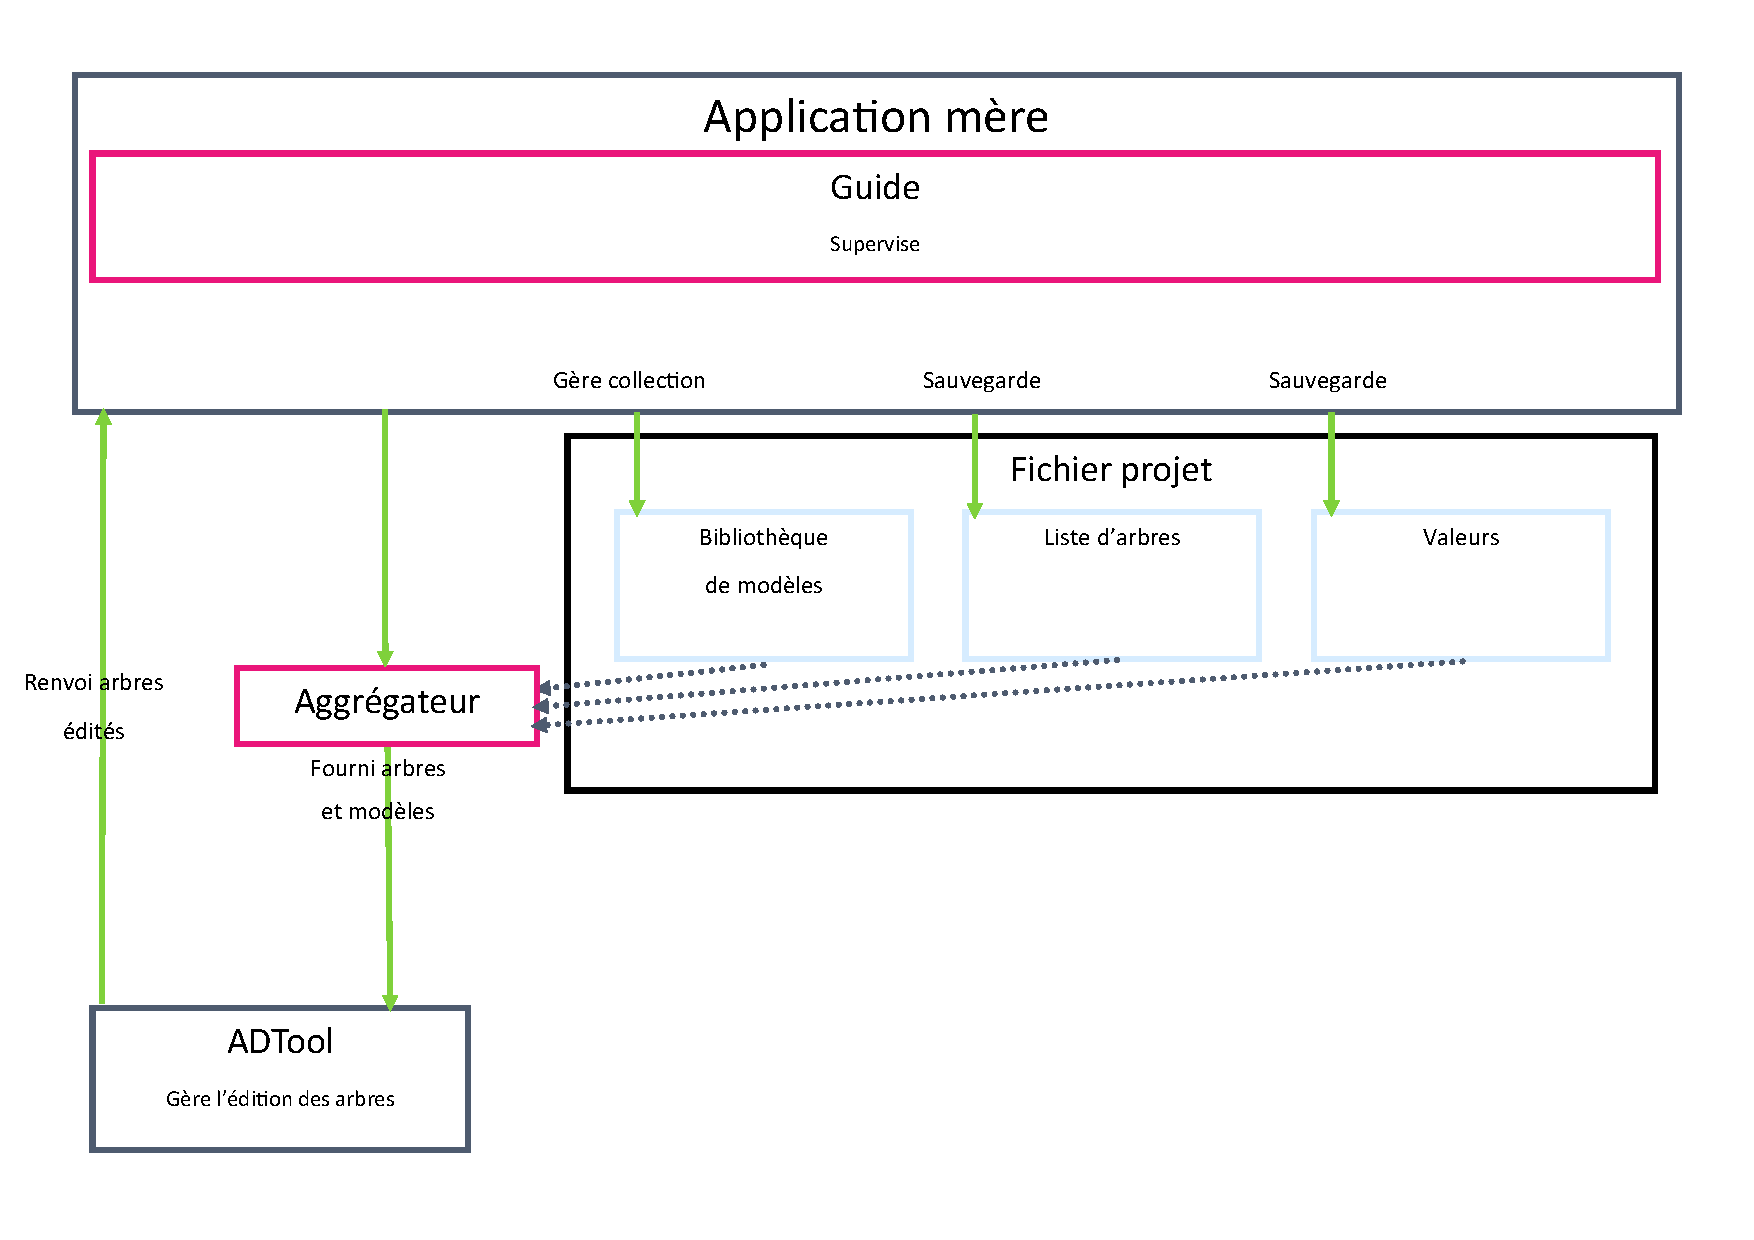
\includegraphics[width=1\textwidth]{figure/archi.pdf}
            \end{center}
            \caption{Différents composants interviendront pour éditer le fichier projet.}
            \label{fig:archi}
        \end{figure}

        Cette bibliothèque sera préchargée à la création du projet. En effet, l'utilisateur devra répondre à une série de questions, qui permettra de sélectionner un sous-ensemble des modèles de la bibliothèque de notre logiciel.

        Comme indiqué par la figure \ref{fig:archi}, ADTool sera un composant de notre application. Il servira à la fois à la visualisation et à l'édition des arbres. Ce choix sera détaillé dans la section \ref{sec:outils}.

        La fonction de synthèse et le filtre seront deux modules différents de l'application. Ils prendront en entrée un arbre du fichier projet (et leurs autres paramètres respectifs), et enverront le résultat à ADTool pour affichage. L'utilisateur décidera ensuite ce qu'il fera de l'arbre généré.

        Le guide (désactivable en option) supervisera l'ensemble de l'application, et devra fournir des informations et consignes pertinentes à l'utilisateur.

    \subsection{Synthèse}
        \label{sec:cahier_synthese}